% anexo_a.tex

\chapter{Anexos}
\label{}



\section{Ejemplo Suma ponderada}\label{ej:sumapond}

Se tienen 3 escenarios posibles indexados por $w = 1,2,3$ y una probabilidad de ocurrencia de cada escenario $w$ igual a $\Theta =(0.5 , 0.3 ,0.2 )$. Para parámetros $c:=(c_{w})_w=(c_1,c_2,c_3)$ y variables de diseño $x:=(x_{w})_w=(x_{1}$, $x_{2}$,$x_{3})$ el valor esperado de la multiplicación entre la variable $x$ y el parámetro $c$ es denotado por $E_{\Theta}[x\cdot c]$
\vspace{2.5mm}

Con esto se tiene la siguiente expresión:

$$E_{\Theta} [ x\cdot c] := x_{1}c_{1}0.5 + x_{2}c_{2}0.3 + x_{3}c_{3}0.2 $$

\section{Parámetros Modelo Original}\label{anexo:parametros}

COMPLETAR

\section{Pruebas iniciales del rendimiento y atención racional en el subastador}\label{anexo:rendimiento}


Para realizar la evaluación del modelo, se realizará un gráfico con los resultados similar a la figura \ref{fig:fig6}. En esta se grafica la cantidad de permisos vendidos por el productor que produce energía con carbón y su influencia en el precio de mercado de los permisos. Esto representa el impacto que puede tener el modelo en eliminar el carbón como productor.

\begin{figure}[H]
    \centering
    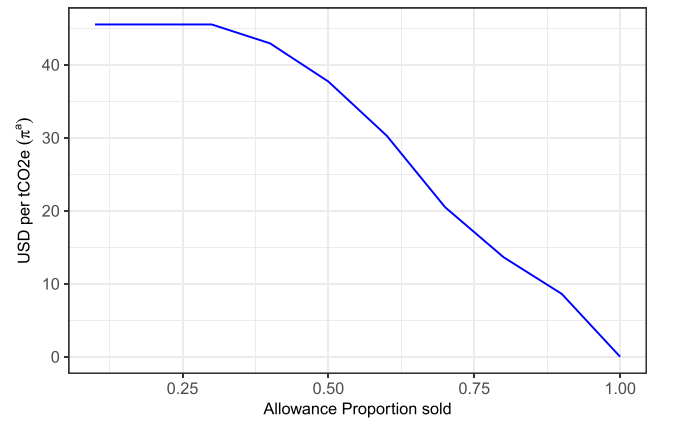
\includegraphics[width=15cm]{docs/DocumentoMemoria/core/images/figura 6 amigo.png}
    \caption{Venta de permisos por generador de carbón (Fuente: \protect\citeB{amigo_two_2021})}
    \label{fig:fig6}
\end{figure}


\subsubsection{Modelo sin restricciones}

Primero se evaluará el modelo al considerar únicamente la función objetivo del subastador con el costo original $\mathcal{F}$ y el costo de rendimiento. También se considera como variable de decisión únicamente los permisos $\theta$.  

\begin{equation}
\begin{array}{rrclcl}
    \displaystyle \min_{\theta} & -\theta \pi^aP + \tilde{\mathcal{F}}(P)+F(\theta)  \label{fo:perfornorest}\\
\end{array}
\end{equation}
\begin{equation}
\begin{array}{cl}
    \theta \geq 0 & (\varrho)
\end{array}
\end{equation}

Con lo anterior se logra el siguiente Lagrangiano:

$$\mathcal{L}(\theta)=-P\theta\pi^a+\mathcal{F}(\theta)+c(P-d)^2 - \varrho\theta $$

Realizando la derivada de primer orden para $\theta$ se obtiene:

\begin{equation}
\begin{array}{rrclcl}
    \frac{\partial\mathcal{L}(\theta)}{\partial (\theta)}=-P\pi^a+\frac{\partial\mathcal{F}(\theta)}{\partial(\theta)}-\varrho=0 \label{lag1}\\
\end{array}
\end{equation}
\begin{equation}
\begin{array}{rrclcl}
    \rightarrow -P\pi^a+\frac{\partial\mathcal{F}(\theta)}{\partial(\theta)}=\varrho \label{lag11}\\
\end{array}
\end{equation}
Con esto se obtiene la siguiente complementariedad para el problema del subastador:

\begin{equation}
\begin{array}{rrclcl}
    0\leq -P\pi^a+\frac{\partial\mathcal{F}(\theta)}{\partial(\theta)}\perp \theta \geq 0 \label{compllag1}\\
\end{array}
\end{equation}

Al igual que en el modelo original de \citeB{amigo_two_2021}, se consideran los siguientes valores para constantes y parámetros:
\begin{enumerate}
    \item $\frac{\partial\mathcal{F}(\theta)}{\partial(\theta)}=0$
    \item $CAP\sim \mathcal{N}(100MtCO_{2}e,0)$
\end{enumerate}

Con esto, al correr el modelo en el \textit{solver}, cambiando únicamente el valor del rendimiento ($P$), se encontraron los siguientes resultados:

\begin{table}[H]
\centering
\begin{tabular}{|l|l|l|}
\hline
\textbf{P($\%$)} & \textbf{$\theta$ (millones)} & \textbf{$\pi^a$($\frac{\$}{\theta}$)} \\ \hline
0 & N/A & N/A \\ \hline
5 & 104 & 223 \\ \hline
10 & 3203 & 0 \\ \hline
15 & 3203 & 0 \\ \hline
20 & 3203 & 0 \\ \hline
25 & 3203 & 0 \\ \hline
30 & 3203 & 0 \\ \hline
35 & 3203 & 0 \\ \hline
40 & 3203 & 0 \\ \hline
45 & 3203 & 0 \\ \hline
50 & 3203 & 0 \\ \hline
55 & 3203 & 0 \\ \hline
60 & 3203 & 0 \\ \hline
65 & 3203 & 0 \\ \hline
70 & 3203 & 0 \\ \hline
75 & 3203 & 0 \\ \hline
80 & 3203 & 0 \\ \hline
85 & 3203 & 0 \\ \hline
90 & 3203 & 0 \\ \hline
95 & 3203 & 0 \\ \hline
100 & 1870 & 0 \\ \hline
\end{tabular}
\caption{Resultados con rendimiento y sin restricciones}
\label{tabla:sinrestr}
\end{table}


Los resultados encontrados en el Cuadro \ref{tabla:sinrestr}, pueden ser resultado de no considerar una restricción para $\theta$ respecto al presupuesto de carbono en el problema del subastador. En la siguiente subsección se desarrolla el problema incluyendo la restricción adicional.

\subsubsection{Modelo con restricción original}

Manteniendo la restricción original de \citeB{amigo_two_2021} mostrada en \ref{res:sub1}. Se tiene el siguiente modelo:

\begin{equation}
\begin{array}{rrclcl}
   \displaystyle \min_{\theta} & -\theta \pi^aP + c(P-d)^2+F(\theta) \\\textrm{s.a.} \label{eq:perforconrestr}\\
\end{array}
\end{equation}
\begin{equation}
\begin{array}{cl}
    \varphi^-1 (\varepsilon )\sigma + \mu - \theta \geq 0 & (\eta)  \label{perforconrestr:r1}
\end{array}
\end{equation}
\begin{equation}
\begin{array}{cl}
    \theta \geq 0 & (\varrho)
\end{array}
\end{equation}

Al igual que el caso anterior, se debe convertir este modelo en un MCP. Para esto se aplican las condiciones de KKT.

$$\mathcal{L}(\theta)=-P\theta\pi^a+\mathcal{F}(\theta)+c(P-d)^2 -\eta(\varphi^-1 (\varepsilon )\sigma + \mu - \theta)- \varrho\theta $$

Realizando la derivada de primer orden para $\theta$ se obtiene:

\begin{equation}
\begin{array}{rrclcl}
    \frac{\partial\mathcal{L}(\theta)}{\partial (\theta)}=-P\pi^a+\frac{\partial\mathcal{F}(\theta)}{\partial(\theta)}-\eta -\varrho=0 \label{lag20}\\
\end{array}
\end{equation}
\begin{equation}
\begin{array}{rrclcl}
    \rightarrow -P\pi^a+\frac{\partial\mathcal{F}(\theta)}{\partial(\theta)}-\eta=\varrho \label{lag21}\\
\end{array}
\end{equation}

Obteniendo la primera complementariedad:

\begin{equation}
\begin{array}{rrclcl}
    0\leq -P\pi^a+\frac{\partial\mathcal{F}(\theta)}{\partial(\theta)}-\eta \perp \theta \geq 0 \label{compllag2}\\
\end{array}
\end{equation}

La segunda complementariedad se obtiene al considera la restricción \ref{perforconrestr:r1} con su variable dual respectiva $\eta$. Obteniendo:

\begin{equation}
\begin{array}{rrclcl}
    0 \leq \varphi^-1 (\varepsilon )\sigma + \mu - \theta \perp \eta \geq 0 \label{compllag21}\\
\end{array}
\end{equation}

Nuevamente, al igual que en el modelo original de \citeB{amigo_two_2021}, se consideran los siguientes valores para constantes y parámetros:
\begin{enumerate}
    \item $\frac{\partial\mathcal{F}(\theta)}{\partial(\theta)}=0$
    \item $CAP\sim \mathcal{N}(100MtCO_{2}e,0)$
\end{enumerate}

Con esto, al correr el modelo en el \textit{solver}, cambiando únicamente el valor del rendimiento ($P$), se encontraron los siguientes resultados:

\begin{table}[H]
\centering
\begin{tabular}{|l|l|l|}
\hline
\textbf{P($\%$)} & \textbf{$\theta$ (millones)} & \textbf{$\pi^a$($\frac{\$}{\theta}$)} \\ \hline
0 & 0.3336 & 30130 \\ \hline
5 & 100 & 315.825 \\ \hline
10 & 100 & 315.825 \\ \hline
15 & 100 & 315.825 \\ \hline
20 & 100 & 315.825 \\ \hline
25 & 100 & 315.825 \\ \hline
30 & 100 & 315.825 \\ \hline
35 & 100 & 315.825 \\ \hline
40 & 100 & 315.825 \\ \hline
45 & 100 & 315.825 \\ \hline
50 & 100 & 315.825 \\ \hline
55 & 100 & 315.825 \\ \hline
60 & 100 & 315.825 \\ \hline
65 & 100 & 315.825 \\ \hline
70 & 100 & 315.825 \\ \hline
75 & 100 & 315.825 \\ \hline
80 & 100 & 315.825 \\ \hline
85 & 100 & 315.825 \\ \hline
90 & 100 & 315.825 \\ \hline
95 & 100 & 315.825 \\ \hline
100 & 100 & 315.825 \\ \hline
\end{tabular}
\caption{Resultados con rendimiento y restricción original}
\label{tabla:conrestr}
\end{table}

Del Cuadro \ref{tabla:conrestr} se entiende que al incluir únicamente las restricciones del problema original solo existe un efecto en el precio y cantidad de permisos cuando el rendimiento es 0. Pero esto no debería ocurrir ya que por lo menos se tiene la información pública $d$. Cabe notar que una cantidad de $100 MtCO_2 e$ con un precio de 315.825 USD cada una, son los valores de resolución del problema original con los mismos parámetros. Este resultado puede resultar debido a que no se a incluido una restricción que describa de mejor forma el costo de rendir.

\section{GAMS de Amigo et al. (2021)}\label{anexo:GAMScomp}
\subsection{MCP del Productor}

\subsubsection{Derivada parcial respecto a $x_i(0)$}

En el código GAMS , se escribió la kkt de esta complementariedad de la siguiente forma en la línea 654:
\begin{verbatim}
kkt_x_first_producer(i).. Inv(i)*(1+percent(i)) + sum(w, psi(i,w))- CF(i)*t_year
*sum(w, sum( tau2,alpha(i,w,tau2))) - xi(i)=g=0;
\end{verbatim}
Siendo xi(i) la variable dual $\xi_i$ . Donde esta kkt se complementa con la variable respectiva $x_i(0)$ en la línea 724 del código.
\begin{verbatim}
kkt_x_first_producer.x_first
\end{verbatim}

\subsubsection{Derivada parcial respecto a $x_i(t,\omega)$}

Al igual que en el caso anterior, el código mantiene la variable dual, se puede ver en la línea 657 del código el KKT respectivo:

\begin{verbatim}
kkt_x_second_producer(i,tau2,w).. ((1/(1+R))**(ord(tau2)))*Prob(w)*Inv(i)*
(1+percent(i))*TCR(i,tau2)- CF(i)*t_year*sum(tau3$(tauAlpha_i(i,tau2,
tau3)),alpha(i,w,tau3)) + psi(i,w) -varphi(i,w,tau2)  =g=0;
\end{verbatim}

Con varphi(i,w,tau2) como la variable dual mencionada $\varphi_{i,\omega,t}$. 

\subsubsection{Derivada parcial respecto a $Q_i(0)$}

Como en los anteriores, en el código no se despeja la variable dual $\lambda_i$, se mantiene y se programa el MCP respectivo con la variable $Q_i(0)$. Se puede ver en la línea 660 del código de la siguiente forma:

\begin{verbatim}
kkt_q1_producer(i,tau).. (int(i)+C(i)*Q_first(i,tau))-pi_d(tau) + kappa(i,tau) - 
lambda(i,tau)+sum(w,gamma(i,w)*epsilon(i))=g= 0;
\end{verbatim}

Programando la complementariedad en la línea 728:

\begin{verbatim}
kkt_q1_producer.Q_first    
\end{verbatim}

\subsubsection{Derivada parcial respecto a $Q_i(t,\omega)$}

La línea 662 del código completa la kkt de la siguiente forma: 

\begin{verbatim}
kkt_qtau_producer(i,tau2,w).. 
((1/(1+R))**(ord(tau2)))*Prob(w)*((TC(i,tau2)*(int(i)+C(i)*Q_second(i,tau2,w)))- 
\end{verbatim}
\begin{verbatim}
pi2_d(tau2,w))+alpha(i,w,tau2)+gamma(i,w)*epsilon(i)-delta(i,tau2,w) =g= 0;
\end{verbatim}

Con la complementariedad escrita de la siguiente forma en la línea 729 del código:
\begin{verbatim}
kkt_qtau_producer.Q_second    
\end{verbatim}

\subsubsection{Derivada parcial respecto a $A_i(t)$}

En el código se tiene lo siguiente en la línea 664:
\begin{verbatim}
   kkt_A_producer(i).. pi_a - sum(w, beta(i,w)) - sum(w, gamma(i,w))=g= 0 
\end{verbatim}

Y efectuando la complementariedad en la línea 730:
\begin{verbatim}
    kkt_A_producer.A
\end{verbatim}

\subsubsection{Derivada parcial respecto a $V_i(w)$}
Programando la kkt en el código en la línea 667:
\begin{verbatim}
    kkt_V_producer(i,w)..  -Prob(w)*pi_v(i,w)+beta(i,w)+gamma(i,w)=g= 0
\end{verbatim}

Completando la complementariedad en la línea 731:
\begin{verbatim}
    kkt_V_producer.V
\end{verbatim}

\subsubsection{Derivada parcial respecto a $P_i(w)$}

Programando la kkt en el código en la línea 670:
\begin{verbatim}
    kkt_P_producer(i,j,w)$(ord(j) <> ord(i))..      Prob(w)* pi_v(j,w)-gamma(i,w) =g= 0
\end{verbatim}

Completando la complementariedad en la línea 732:
\begin{verbatim}
    kkt_P_producer.P  
\end{verbatim}

\subsubsection{Completando el problema del productor}

Las cuales se encuentran programadas entre las líneas 609 y 703 del código:

\begin{verbatim}
    capacity_stage_2_xnext(i,w,tau2).. CF(i)*t_year*(sum(tau3$(tau3_i(i,tau2,tau3)),
    x_next(i,tau3,w))+x_first(i)+Q_barT2(i,tau2) +Q_bar(i))-Q_second(i,tau2,w) =g=0;
\end{verbatim}
\begin{verbatim}
    capacity_stage_1(i,tau)..  CF(i)*t_year*Q_bar(i)- Q_first(i,tau) =g=0;
\end{verbatim}
\begin{verbatim}
    trading_permits(i,w)..  A(i)-V(i,w) =g= 0;
\end{verbatim}
\begin{verbatim}
    total_allowances(i,w)..  A(i) + sum(j$(ord(j) <> ord(i)),P(i,j,w))-V(i,w) - 
    sum(tau2,Q_second(i,tau2,w)*epsilon(i)) - sum(tau,Q_first(i,tau)*epsilon(i))   
    =g= 0;
\end{verbatim}
\begin{verbatim}
    resource_potential(i,w)..   -Q_bar(i) - x_first(i) - sum(tau3,x_next(i,tau3,w))+
    sum(tau2,Q_barT2(i,tau2)) + RP(i) =g= 0;
\end{verbatim}

Existiendo sus complementariedades entre las líneas 734 y 744:

\begin{verbatim}
    capacity_stage_1.kappa
    capacity_stage_2_xnext.alpha
    resource_potential.psi
    trading_permits.beta
\end{verbatim}

\subsection{MCP condiciones de mercado}

\subsubsection{Restricción de permisos disponibles}
En el código se encuentra la restricción y complementariedad en las líneas 708 y 751 respectivamente: 
\begin{verbatim}
    kkt_A_theta..    theta - sum(i,A(i))=e= 0;
    kkt_A_theta.pi_a
\end{verbatim}

\subsubsection{Restricción de equilibrio en el mercado de compra y venta de permisos}
En el código se encuentra la restricción y complementariedad en las líneas 713 y 752 respectivamente: 
\begin{verbatim}
    kkt_P_V(i,w).. V(i,w)=e=sum(j$(ord(j) <> ord(i)),P(j,i,w));
    kkt_P_V.pi_v 
\end{verbatim}

\subsubsection{Abastecimiento de demanda en la primera etapa}
\begin{verbatim}
    kkt_Q_D_first(tau).. sum(i,Q_first(i,tau))=e=D1(tau);
    kkt_Q_D_first.pi_d
\end{verbatim}

\subsubsection{Abastecimiento de demanda en la segunda etapa}
En el código se encuentra la restricción y complementariedad en las líneas 711 y 754 respectivamente: 
\begin{verbatim}
    kkt_Q_D_second(tau2,w)..sum(i,Q_second(i,tau2,w))=e=D2(w,tau2);
    kkt_Q_D_second.pi2_d
\end{verbatim}


\section{Aproach inicial: Reordenando modelo del subastador con función de costo diferenciable}\label{Anexo:aproachinicial}

Se define el \emph{performance} óptimo para el premio ($R = \theta \pi^a$). Donde el \emph{performace} óptimo  se define como $P^*(r) = (C')^{-1}(r)$ de la siguiente forma:

\begin{equation}
\begin{array}{rrclcl}
    P^*(\theta \pi^a) = \begin{cases}\frac{\theta \pi^a}{2c}+d,&\theta \pi^a\leq 2c(1-d)\\1,&\theta \pi^a>2c(1-d)\end{cases}, \label{performaceoptimo}\\
\end{array}
\end{equation}

\citeB{dewan_estimating_2020} propone la opción de agregar una función de costo asociada al \textit{performance}(rendimiento en inglés) de obtener la variable de decisión (en este caso $\theta$) lo más cercana a la óptima al invertir en investigación que mejore la estimación de la variable.
\vspace{2.5mm}

Considerando \ref{nuevafposible}, tomando $Pr(\theta\leq CAP) = P$ con $P : $\textit{performance}, la función objetivo del subastador puede reorganizarse de la siguiente forma:

\begin{equation}
\begin{array}{rrclcl}
    \displaystyle \min_{\theta,P} & -\theta \pi^aP + \tilde{\mathcal{F}}(P)+F(\theta)  \label{fo:performance0}\\
\end{array}
\end{equation}

Para completar el problema de optimización se debe definir ciertos supuesto. Para comenzar, se debe definir que factores serán variables y parámetros. Por el momento, se asume que la única variable es $\theta$ y el subastador busca un \textit{performace} mayor al umbral de información pública.  
\vspace{2.5mm}

Entonces, debe identificarse $\tilde{\mathcal{F}}(P)$ de acuerdo a su definición en \ref{costoperformace} cuando se cumple que el \textit{performace} es mayor al umbral de información pública $d$ entonces se define lo siguiente, conociendo los parámetros $c, d$:

$$\tilde{\mathcal{F}}(P)=c(P-d)^2$$ 

De esto se deben definir las restricciones del problema. La primera corresponde a la positividad de $\theta$. 

\begin{equation}
\begin{array}{cl}
    \theta \geq 0 & (\varrho)\label{res:newsub1}
\end{array}
\end{equation}

Para la segunda, se debe aplicar la función de \textit{performance} óptimo para el ingreso \ref{performaceoptimo}. La idea es encontrar una restricción para definir este problema teniendo solo a $\theta$ como variable.  Entonces la opción es aplicar la siguiente restricción: 

\begin{equation}
\begin{array}{cl}
    \theta \pi^a\leq 2c(1-d) & (\eta) \label{res:newsub2}
\end{array}
\end{equation}

Con esto el problema del subastador quedaría reformulado de la siguiente manera:

\begin{equation}
\begin{array}{rrclcl}
    \displaystyle \max_{\theta} & \theta \pi^a(\frac{\theta \pi^a}{2c}+d) - c((\frac{\theta \pi^a}{2c}+d)-d)^2  \\\textrm{s.a.}\\
\end{array}
\end{equation}
\begin{equation}
\begin{array}{cl}
    \theta \pi^a\leq 2c(1-d) & (\eta) 
\end{array}
\end{equation}
\begin{equation}
\begin{array}{cl}
    \theta \geq 0 & (\varrho)
\end{array}
\end{equation}

\subsubsection{Maximizando el rendimiento}

Esta formulación es considerada completa en un contexto donde, al igual que el trabajo original, se quiere maximizar los \textit{allowances} (permisos de contaminación) para la industria generadora. Pero, en esta memoria, se busca reordenar el problema donde el subastador sufra perdidas por su mala gestión, intentando mejorar su rendimiento.
\vspace{2.5mm}

Para lograr lo anterior, es necesario definir el problema tomando como variable de decisión el rendimiento ( \textit{performance}). Con esto, es necesario definir la variable $P$ respecto a $\theta$ para que poder utilizar el problema en el modelo general al incluir a el problema de los productores(generadores de electricidad).
\vspace{2.5mm}

Luego, de \ref{res:newsub2} y \ref{performaceoptimo} se obtiene la siguiente igualdad:

$$P^*(\theta \pi^a) = \frac{\theta \pi^a}{2c}+d$$

Si se despeja $P$ se obtiene su valor respecto a $\theta$:

$$\theta=\frac{(P-d)2c}{\pi^a}$$

Despejando esta variable en \ref{fo:performance0}, se obtiene la siguiente función objetivo:


\begin{equation}
\begin{array}{rrclcl}
    \displaystyle \max_{P} & \frac{(P-d)2c}{\pi^a} \pi^{a}P - c(P-d)^2  \label{fo:3}\\
\end{array}
\end{equation}

La cuál se puede simplificar llegando a lo siguiente:

\begin{equation}
\begin{array}{rrclcl}
    \displaystyle \max_{P} & c(P^{2}-d^{2}) \label{fo:4}\\
\end{array}
\end{equation}

La cuál tiene sentido pero no es aplicable en el trabajo de \citeB{dewan_estimating_2020}, ya que según la proposición 4, descrita en \ref{marco:costos}, el problema de maximización debe ser cóncavo. Pero debido a la forma en la que se definió el premio ($r=\pi^{a}\theta$), la concavidad de la función de costo en este caso no transforma \ref{fo:4} en cóncava. Debido a esto, no se puede encontrar un máximo local que sea también un máximo global en el problema que comprueba la proposición 4.
\vspace{2.5mm}


Para lograr la concavidad necesaria, se encuentra la posibilidad de incorporar un elemento del problema original del subastador. Con esto, además de cumplir con la proposición 4, se expande el alcance de este trabajo, ya que ahora no solo se está reordenado el problema al aplicar un sistema nuevo de incentivo, si no que, se incorpora el costo mencionado en el trabajo originial de AMIGO llamado Costo Social del Carbón (SCC). Con esto amplía el estudio para definir este costo respecto al rendimiento del subastador.
\vspace{2.5mm}

La primera aplicación de este costo es la de entender que el costo SCC dependerá de los permisos emitidos, ya que a mayor cantidad de permisos, existirá mayor costos asociados al uso del carbón. Por lo que, inicialmente, se  define el SCC como: $F(\theta)= \alpha\theta + \beta$ ($\alpha$,$\beta$ parámetros). 
\vspace{2.5mm}

Luego, la idea es que este costo transforme \ref{fo:4} a una función cóncava, por lo que se debe cumplir lo siguiente:

\begin{equation}
\begin{array}{rrclcl}
    F(\theta)= \alpha\theta + \beta = kP^2 \label{fo:5}\\
\end{array}
\end{equation}

Donde, si $k>c$ (de \ref{fo:4}), se logra una función objetivo cóncava. Obteniendo, luego de reemplazar la variable de permisos $\theta$ por su valor en función del rendimiento $P$, la siguiente función de costo social a incorporar en el modelo:

\begin{equation}
\begin{array}{rrclcl}
    F(\frac{(P-d)2c}{\pi^a})= \alpha\frac{(P-d)2c}{\pi^a} + \beta = kP^2 \\
\end{array}
\end{equation}

De la cuál, se deben encontrar los valores de $\alpha$ y $\beta$ que cumplan con la igualdad.




\section{Resultados modelo \textit{Profit Oriented}} \label{anexoPO}


\begin{table}[H]
    \centering
    \begin{tabular}{|l|l|l|l|l|}
    \hline
        Rend[P]  & CAP & $\theta$  & $\frac{\theta}{CAP}$  & $\pi^a$ \\ \hline
        0.798 & 100,000,000.000 & 120,200,000.000 & 1.20 &  \$270.13  \\ \hline
        0.8 & 100,000,000.000 & 120,200,000.000 & 1.20 &  \$270.13  \\ \hline
        0.85 & 100,000,000.000 & 113,654,321.432 & 1.14 &  \$25.75  \\ \hline
        0.9 & 100,000,000.000 & 113,568,965.603 & 1.14 &  \$93.65  \\ \hline
        0.95 & 100,000,000.000 & 118,470,479.300 & 1.18 &  \$188.86  \\ \hline
        0.99 & 100,000,000.000 & 114,916,396.444 & 1.15 &  \$298.11  \\ \hline
        1 & 100,000,000.000 & 118,332,486.090 & 1.18 &  \$317.24  \\ \hline
        0.798 & 200,000,000.000 & 240,400,000.000 & 1.20 &  \$161.56  \\ \hline
        0.8 & 200,000,000.000 & 240,400,000.000 & 1.20 &  \$60.57  \\ \hline
        0.85 & 200,000,000.000 & 229,255,128.800 & 1.15 &  \$12.77  \\ \hline
        0.9 & 200,000,000.000 & 223,154,111.799 & 1.12 &  \$47.66  \\ \hline
        0.95 & 200,000,000.000 & 234,207,864.377 & 1.17 &  \$95.53  \\ \hline
        0.99 & 200,000,000.000 & 224,918,654.768 & 1.12 &  \$152.31  \\ \hline
        1 & 200,000,000.000 & 226,010,004.000 & 1.13 &  \$166.10  \\ \hline
        0.798 & 300,000,000.000 & 360,600,000.000 & 1.20 &  \$119.47  \\ \hline
        0.8 & 300,000,000.000 & 360,600,000.000 & 1.20 &  \$119.47  \\ \hline
        0.85 & 300,000,000.000 & 356,171,492.939 & 1.19 &  \$2,083.93  \\ \hline
        0.9 & 300,000,000.000 & 360,600,000.000 & 1.20 &  \$13,948,075.51  \\ \hline
        0.95 & 300,000,000.000 & 268,982,380.464 & 0.90 &  \$83.18  \\ \hline
        0.99 & 300,000,000.000 & 313,308,201.957 & 1.04 &  \$109.34  \\ \hline
        1 & 300,000,000.000 & 313,402,369.287 & 1.04 &  \$119.78  \\ \hline
        0.798 & 400,000,000.000 & 480,800,000.000 & 1.20 &  \$95.83  \\ \hline
        0.8 & 400,000,000.000 & 454,798,037.400 & 1.14 &  \$95.83  \\ \hline
        0.85 & 400,000,000.000 & 480,800,000.000 & 1.20 &  \$10,345,937.92  \\ \hline
        0.9 & 400,000,000.000 & 480,800,000.000 & 1.20 &  \$22.12  \\ \hline
        0.95 & 400,000,000.000 & 268,982,380.500 & 0.67 &  \$83.18  \\ \hline
        0.99 & 400,000,000.000 & 404,778,933.700 & 1.01 &  \$84.63  \\ \hline
        1 & 400,000,000.000 & 362,299,397.300 & 0.91 &  \$103.62  \\ \hline
        0.798 & 500,000,000.000 & 601,000,000.000 & 1.20 &  \$79.31  \\ \hline
        0.8 & 500,000,000.000 & 601,000,000.000 & 1.20 &  \$79.31  \\ \hline
        0.85 & 500,000,000.000 & 601,000,000.000 & 1.20 &  \$7.78  \\ \hline
        0.9 & 500,000,000.000 & 601,000,000.000 & 1.20 &  \$47.07  \\ \hline
        0.95 & 500,000,000.000 & 268,982,577.800 & 0.54 &  \$83.18  \\ \hline
        0.99 & 500,000,000.000 & 551,200,775.300 & 1.10 &  \$62.15  \\ \hline
        1 & 500,000,000.000 & 274,684,779.400 & 0.55 &  \$136.66  \\ \hline
\end{tabular}
\end{table}

\begin{table}[H]
    \centering
    \begin{tabular}{|l|l|l|l|l|}
    \hline
        Rend[P]  & CAP & $\theta$  & $\frac{\theta}{CAP}$  & $\pi^a$ \\ \hline
        0.798 & 600,000,000.000 & 721,200,000.000 & 1.20 &  \$66.57  \\ \hline
        0.8 & 600,000,000.000 & 605,279,898.700 & 1.01 &  \$66.57  \\ \hline
        0.85 & 600,000,000.000 & 721,200,000.000 & 1.20 &  \$66.57  \\ \hline
        0.9 & 600,000,000.000 & 578,230,501.600 & 0.96 &  \$6,546.01  \\ \hline
        0.95 & 600,000,000.000 & 268,982,577.800 & 0.45 &  \$83.18  \\ \hline
        0.99 & 600,000,000.000 & 719,988,509.800 & 1.20 &  \$47.58  \\ \hline
        1 & 600,000,000.000 & 274,684,779.400 & 0.46 &  \$136.66  \\ \hline
        0.798 & 700,000,000.000 & 841,400,000.000 & 1.20 &  \$56.37  \\ \hline
        0.8 & 700,000,000.000 & 605,279,898.700 & 0.86 &  \$56.37  \\ \hline
        0.85 & 700,000,000.000 & 790,095,058.700 & 1.13 &  \$56.37  \\ \hline
        0.9 & 700,000,000.000 & 181,880,800.200 & 0.26 &  \$105.13  \\ \hline
        0.95 & 700,000,000.000 & 268,982,854.700 & 0.38 &  \$83.18  \\ \hline
        0.99 & 700,000,000.000 & 275,744,578.300 & 0.39 &  \$14,670.45  \\ \hline
        1 & 700,000,000.000 & 212,794,913.300 & 0.30 &  \$3,786,269.25  \\ \hline
        0.798 & 800,000,000.000 & 961,600,000.000 & 1.20 &  \$48.76  \\ \hline
        0.8 & 800,000,000.000 & 961,600,000.000 & 1.20 &  \$152.50  \\ \hline
        0.85 & 800,000,000.000 & 790,095,058.700 & 0.99 &  \$152.50  \\ \hline
        0.9 & 800,000,000.000 & 181,880,800.200 & 0.23 &  \$105.13  \\ \hline
        0.95 & 800,000,000.000 & 268,982,577.800 & 0.34 &  \$83.18  \\ \hline
        0.99 & 800,000,000.000 & 275,744,735.700 & 0.34 &  \$14,665.37  \\ \hline
        1 & 800,000,000.000 & 212,794,913.339 & 0.27 &  \$3,786,269.25  \\ \hline
        0.798 & 900,000,000.000 & 1,081,800,000.000 & 1.20 &  \$42.26  \\ \hline
        0.8 & 900,000,000.000 & 605,279,898.700 & 0.67 &  \$42.26  \\ \hline
        0.85 & 900,000,000.000 & 790,095,058.700 & 0.88 &  \$42.26  \\ \hline
        0.9 & 900,000,000.000 & 181,880,800.200 & 0.20 &  \$105.13  \\ \hline
        0.95 & 900,000,000.000 & 268,982,577.800 & 0.30 &  \$83.18  \\ \hline
        0.99 & 900,000,000.000 & 275,744,846.500 & 0.31 &  \$14,661.80  \\ \hline
        1 & 900,000,000.000 & 212,794,913.300 & 0.24 &  \$3,786,269.25  \\ \hline
        0.798 & 1,000,000,000.000 & 1,202,000,000.000 & 1.20 &  \$35.98  \\ \hline
        0.8 & 1,000,000,000.000 & 605,279,898.700 & 0.61 &  \$35.98  \\ \hline
        0.85 & 1,000,000,000.000 & 790,095,058.700 & 0.79 &  \$35.98  \\ \hline
        0.9 & 1,000,000,000.000 & 181,880,800.200 & 0.18 &  \$105.13  \\ \hline
        0.95 & 1,000,000,000.000 & 268,982,577.800 & 0.27 &  \$83.18  \\ \hline
        0.99 & 1,000,000,000.000 & 275,794,121.000 & 0.28 &  \$124.41  \\ \hline
        1 & 1,000,000,000.000 & 212,794,913.300 & 0.21 &  \$3,786,269.25 \\ \hline
    \end{tabular}
    \caption{Efecto de P en $\theta$ y $\pi^a$ para todo CAP}
    \label{efectopenthetapiatodoCAP}
\end{table}


